\chapter{Introduction}
\emph{The Java Modelling Tools} (JMT) is a free open source suite
consisting of \emph{six} tools  for performance evaluation,
capacity planning, workload characterization, and modelling of
computer and communication systems. The suite implements several
state-of-the-art algorithms for the exact, asymptotic and
simulative analysis of queueing network models, either with or
without product-form solution. Models can be described either
through \emph{wizard} dialogs or with a \emph{graphical}
user-friendly interface. The workload analysis tool is based on
clustering techniques. The suite incorporates an XML data layer
that enables full reusability of the computational engines.

\medskip \noindent 
\includegraphics[scale=.5]{img/JSIMIcon}
\textbf{JSIM\emph{wiz}:} a wizard-based interface for the
discrete-event simulator JSIM for the analysis of queueing network
models. A sequence of \emph{wizard} windows helps for the
definition of the network properties. The JSIM simulation engine
supports several probability distributions for characterizing
service and inter-arrival times. Load-dependent strategies using
arbitrary functions of the current queue-length can be specified.
JSIM\emph{wiz} supports state-independent routing strategies,
e.g., Markovian or round robin, as well as state-dependent
strategies, e.g., routing to the server with minimum utilization,
or with the shortest response time, or with minimum queue-length.
The simulation engine supports several extended features not
allowed in product-form models, namely, Finite Capacity Regions
(i.e., blocking), fork-join servers (i.e., parallelism), and
priority classes. The JSIM perform automatically the transient
detection, based on spectral analysis, compute and plot on-line
the values with the confidence intervals. What-if analyses, where
a sequence of simulations is run for different values of control
parameters, are also possible.

\medskip \noindent 
\includegraphics[scale=.5]{img/JMODELIcon}
\textbf{JSIM\emph{graph}:} a \emph{graphical} user-friendly
interface for the same simulator engine JSIM used by
JSIM\emph{wiz}. It integrates the same functionalities of
JSIM\emph{wiz} with an intuitive graphical workspace. This allows
an easy description of network structure, as well as a simplified
definition of the input and execution parameters. Network
topologies can be exported in vectorial or raster image formats.

\medskip \noindent 
\includegraphics[scale=.5]{img/JMVAIcon}
\textbf{JMVA:} for the \emph{exact} analysis of single-class or
multiclass product-form queueing networks, processing \emph{open,
closed} or \emph{mixed} workloads. A stabilized version of the
Mean Value Analysis MVA algorithm is used. Network structure is
specified by textual \emph{wizards}. What-if analyses and
graphical representation of the results are provided.

\medskip \noindent 
\includegraphics[scale=.5]{img/JMCHIcon}
\textbf{JMCH:} it applies a simulation technique to solve a single
station model, with finite (M/M/1/k) or infinite queue (M/M/1),
and shows the underlying Markov Chain. It is possible to
dynamically change the arrival rate and service time of the
system.

\medskip \noindent 
\includegraphics[scale=.5]{img/JABAIcon}
\textbf{JABA:} for the identification of \emph{bottlenecks} in
multiclass closed product-form networks using efficient convex
hull algorithms. Up to three customer classes are supported. It is
possible to identify potential bottlenecks corresponding to the
different mixes of customer classes in execution. Models with
thousands of queues can be analyzed efficiently.
\emph{Optimization} studies (e.g., throughput maximization,
minimization of response time, identification of the optimal load)
can be performed through the identification of the
\emph{saturation sectors}, i.e., the mixes of customer classes in
execution that saturate more than one resource simultaneously.

\medskip \noindent 
\includegraphics[scale=.5]{img/JWATIcon}
\textbf{JWAT:} supports the \emph{workload characterization}
process. Some standard formats for input file are provided (e.g.,
Apache HTTP and IIS log files), customized formats may also be
specified. The imported data can initially be analyzed using
descriptive statistical techniques (e.g, means, correlations,
histograms, boxplots, scatterplots), either for univariate or
multivariate data. Algorithms for data scaling, sample extraction,
outlier filtering, k-means and fuzzy k-means clustering for
identifying similarities in the input data are provided. These
techniques allow the identification of cluster of customers having
similar characteristics. The clusters centroids represent the mean
values of the parameters of the classes (e.g., CPU time, n.o of
I/Os, n.o of web pages pages accessed) that can be used for the
workload parametrization. The tool includes an interface to the
similarity clustering tool CLUTO.

\section{Starting with the JMT suite}
Double click on the JMT icon

\includegraphics[scale=.5]{img/JMTIcon} on your \emph{program group} or
on the \emph{desktop}, or open the \emph{command prompt} and type
from the installation directory:
\begin{verbatim}
    java -jar JMT.jar
\end{verbatim}
The window of \autoref{fig:startscreen} will be shown.

\begin{figure}[htbp]
    \begin{center}
        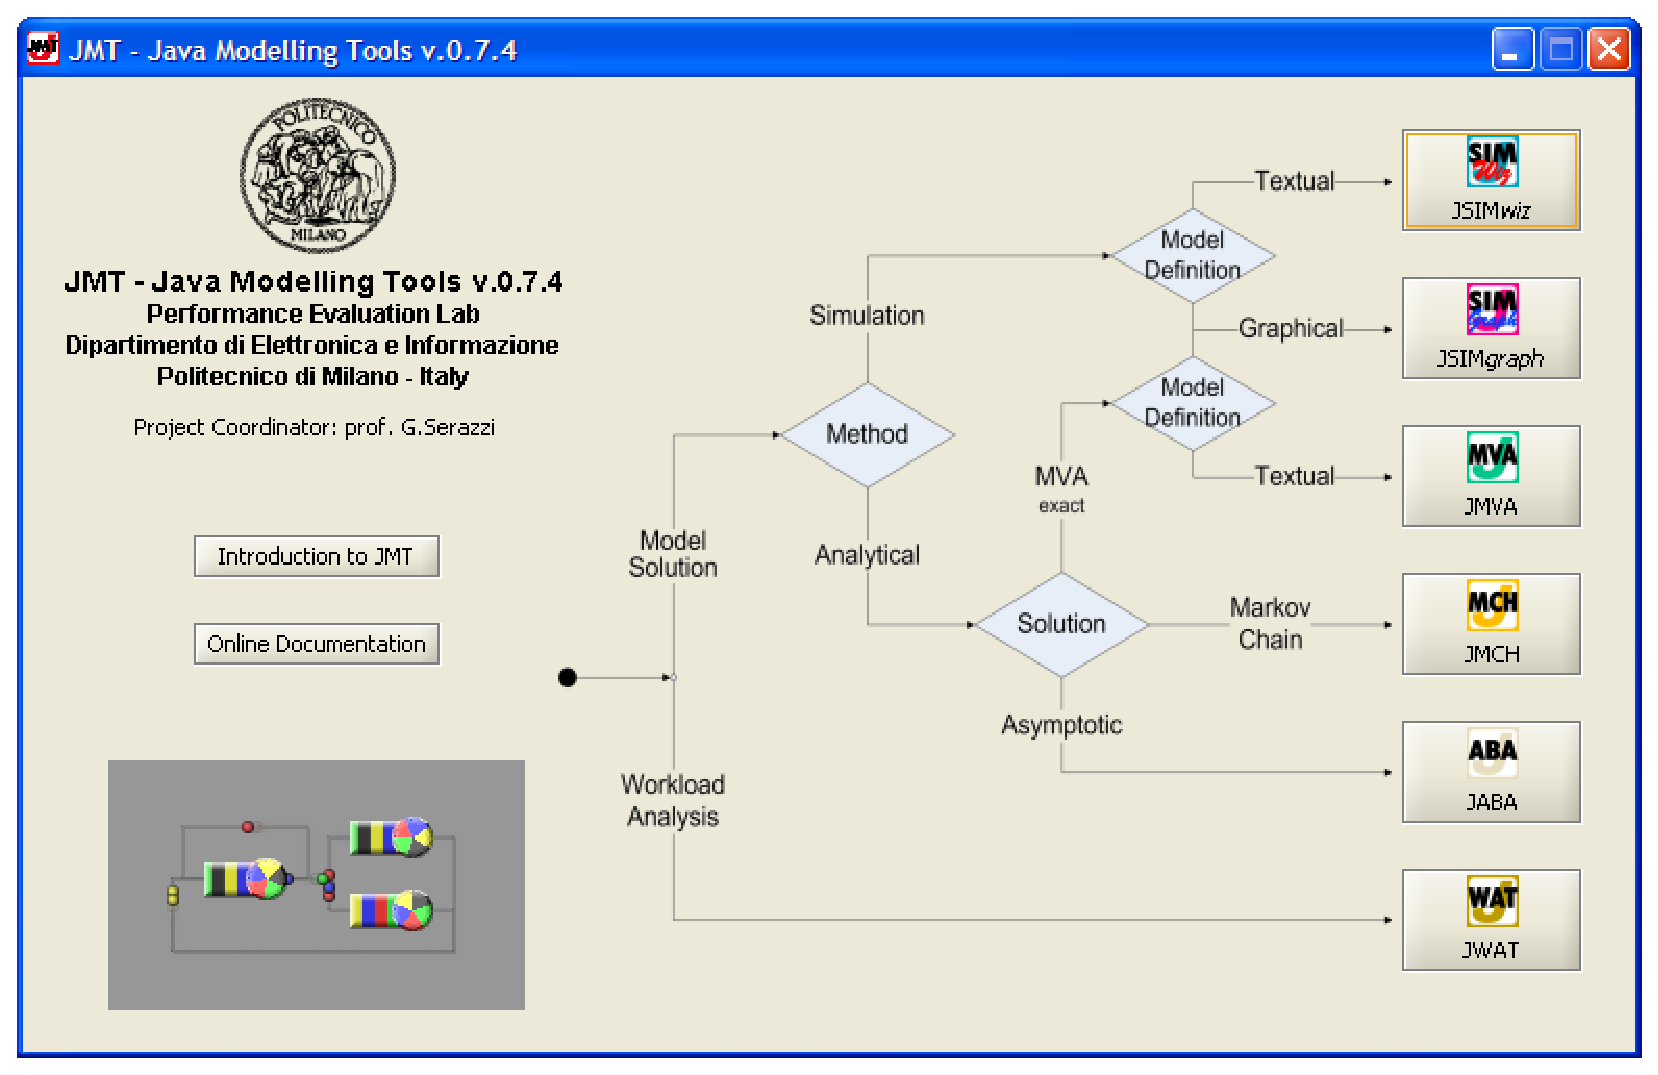
\includegraphics[scale=.5]{img/StartScreen}
    \end{center}
    \caption{The JMT suite Starting Screen}
    \label{fig:startscreen}
\end{figure}

This starting screen is used to select the application of the
suite to be executed by clicking on the corresponding button. The
flow chart should help the user to select the application that
best fits its needs.

In the following chapters the tools will be examined in details
and some examples are given. This manual is intended for the
general user that wants to learn how to interact with JMT.
Advanced users that want to learn details on internal data
structures, computational engines and XML interfaces should refer
to \emph{JMT system manual}.\\
Several other documents related to JMT description and
applications are provided with the suite. Click on \texttt{Online
Documentation} button to access the library. An exercise
book is also available.\\

\textbf{We hope you will find this material of some help and
apologize in advance for the mistakes you will find. }
